\documentclass[journal,12pt,twocolumn]{IEEEtran}
\usepackage[none]{hyphenat}
\usepackage{enumitem}
\usepackage{graphics}
\usepackage{graphicx}
\usepackage{listings}
\usepackage{ragged2e}
\usepackage{kvmap}
\usepackage{multirow}
\usepackage[english]{babel}
\usepackage{caption}
\usepackage{tikz}
\usetikzlibrary{arrows,shapes,automata,petri,positioning,calc}


\title{ MULTIPLE SEQUENCE DETECTOR 1100 and 0100}
\author{Ganga Gopinath}
\date{August 2022}

\begin{document}

\maketitle
\begin{tableofcontents}
\begin{abstract}
This manual explains state machines by identify the sequence that detect 1100 and 0100
\end{abstract}
\section{Components}

\vspace{0.2cm}

\begin{table}[h]
\centering

\begin{tabular}{|c|c|c|}
\hline
Components & Value & Quantity\\
\hline
Resistor & 220 Ohm & 1\\
\hline
Arduino & UNO & 1\\
\hline
Seven Segment Display & & 1\\
\hline
Decoder & 7447 & 1\\
\hline
Flip Flop & 7474 & 2\\
\hline
Bread Board & & 1\\
\hline
Jumper Wires & & 20\\
\hline
\end{tabular}
\vspace{2mm}
%\caption{.0}
\label{table:1}
\end{table}
\section{sequence detector}
  A sequence detector accepts as input a string of bits: either 0 or 1. Its output goes to 1 when a target sequence has been detected.There are two basic types:  overlap  and  non-overlap. In a sequence detector that allows overlap, the final bits of one sequence can be  the start of another sequence.  Our examples 1100 and 0100 sequence detector.  It raises an output of 1 when the last 4 binary bits received 1100 or 0100.
  \newline
\subsection{\textbf{STATE DIAGRAM}}
State diagrams are used to give an abstract description of the behavior of a system. This behavior is represented as a series of events that can occur in one or more possible states.State diagram is represented in Figure 1
\begin{figure}
%{\includegraphics[scale=.5]{../assign/statediagram.png} 
 %\includegraphics[scale=.5]{../../assign/statediagram.png} 
 
 
 
 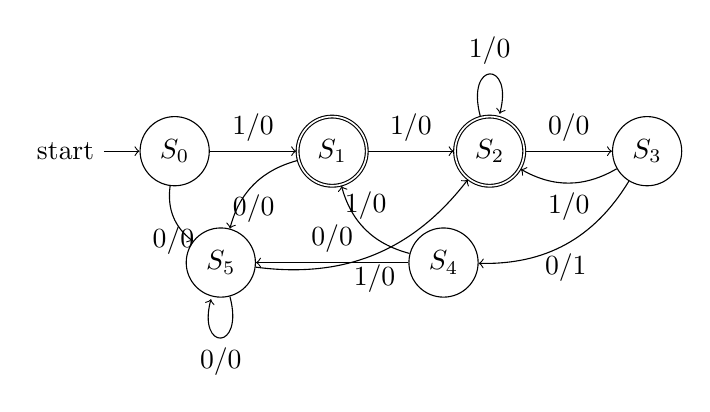
\begin{tikzpicture} [node distance=2cm]
\node[circle, draw, state, initial] (S0) {$S_0$};
\node[circle, draw, state, accepting, right of=S0] (S1) {$S_1$};
\node[circle, draw, state, accepting, right of=S1] (S2) {$S_2$};
\node[circle, draw, state, below left of = S1] (S5) {$S_5$};
\node[circle, draw, state, below right of = S1] (S4) {$S_4$};
\node[circle, draw, state, right of=S2] (S3) {$S_3$};
\path[->] (S0) edge[above] node{1/0} (S1)
          (S1) edge[above] node{1/0} (S2)
          (S2) edge[above] node{0/0} (S3)
          
          (S4) edge[above] node{0/0} (S5)
          (S2) edge[loop above] node{1/0} (S2)
          (S5) edge[loop below] node{0/0} (S5)
          (S0) edge[below,bend right] node{0/0} (S5)
          (S5) edge[below,bend right] node{1/0} (S2)
          (S1) edge[below,bend right] node{0/0} (S5)
          (S3) edge[below,bend left] node{1/0} (S2)
          (S4) edge[above,bend left] node{1/0} (S1)
          (S3) edge[below,bend left] node{0/1} (S4); 
\end{tikzpicture}
\begin{center}
\caption{State Diagram for Sequence}
 \label{Fig 1}
\end{center}
 
\end{figure}

\vspace{5mm}
\subsection{\textbf{STATE TABLE}}
  From state diagram,state table can be generated in Table II.
  
  \vspace{5mm}
  \begin{table}[h]
\centering
  \begin{tabular}{|c|c|c|c|}
   \hline
   
   \textbf{Present State}&{Input}&{Next state}&{Output}\\
   \hline
   
   \textbf{S0}& {0}&{S5}&{0}\\
   \textbf{S0}&{1}&{S1}&{0}\\
   \textbf{S1}& {0}&{S5}&{0}\\
   \textbf{S1}&{1}&{S2}&{0}\\
   \textbf{S2}&{0}&{S3}&{0}\\
   \textbf{S2}&{1}&{S2}&{0}\\
   \textbf{S3}&{0}&{S4}&{1}\\
   \textbf{S3}&{1}&{S4}&{0}\\
   \textbf{S4}&{0}&{S5}&{0}\\
   \textbf{S4}&{1}&{S1}&{0}\\
   \textbf{S5}&{0}&{S5}&{0}\\
   \textbf{S5}&{1}&{S2}&{0}\\
   \hline
   \hline
  \end{tabular}
  
  \vspace{10mm}
  
\caption{.STATE TABLE}
\label{table:2}
  `\end{table}

 \subsection{\textbf{TRUTH TABLE}}
  
  \vspace{5mm}
  \begin{table}[h]
\centering
  \begin{tabular}{|c|c|c|c|}
   \hline
   
   \textbf{Present State}&{Input}&{Next state}&{Output}\\
   \hline
   \textbf{A B C}&{X}&{P Q R}&{Y}\\
   \textbf{0 0 0}& {0}&{1 0 1}&{0}\\
   \textbf{0 0 0}&{1}&{0 0 1}&{0}\\
   \textbf{0 0 1}& {0}&{1 0 1}&{0}\\
   \textbf{0 0 1}&{1}&{0 1 0}&{0}\\
   \textbf{0 1 0}&{0}&{0 1 1}&{0}\\
   \textbf{0 1 0}&{1}&{0 1 0}&{0}\\
   \textbf{0 1 1}&{0}&{1 0 0}&{1}\\
   \textbf{0 1 1}&{1}&{0 1 0}&{0}\\
   \textbf{1 0 0}&{0}&{1 0 1}&{0}\\
   \textbf{1 0 0}&{1}&{0 0 1}&{0}\\
   \textbf{1 0 1}&{0}&{1 0 1}&{0}\\
   \textbf{1 0 1}&{0}&{0 1 0}&{0}\\
   \hline
   \hline
  \end{tabular}
  
  \vspace{10mm}
  
\caption{.TRUTH TABLE}
\label{table:3}
  `\end{table}

  
  \newpage
  
  \subsection{\textbf{Karnaugh Map } }
  
  \begin{kvmap}
    \begin{kvmatrix}{C,X,A,B}
    1 & 0 & 0 & 1\\
    0 & 0 & 0 & 1\\
    X & X & X & X\\
    1 & 0 & 0 & 1\\
    \end{kvmatrix}
    \bundle[color=green ,invert=true,overlapmargins=8pt]{3}{0}{3}{3}
    \bundle[color=green ,invert=true,overlapmargins=8pt]{0}{0}{0}{3}
  
    \bundle[color=red]{3}{0}{2}{3}
\end{kvmap}
\newline
\begin{equation}
    P=B'X'+CX'
    \label{eq1}
\end{equation}
 
  \begin{kvmap}
    \begin{kvmatrix}{C,X,A,B}
    0 & 0 & 1 & 0\\
    1 & 1 & 1 & 0\\
    X & X & X & X\\
    0 & 0 & 1 & 0\\
    \end{kvmatrix}
    \bundle[color=red]{2}{0}{2}{3}
    \bundle[color=green]{0}{1}{1}{2}
    
    
\end{kvmap}
\begin{equation}
    Q= CX+BX'
    \label{eq2}
\end{equation}

 \begin{kvmap}
    \begin{kvmatrix}{C,X,A,B}
    1 & 1 & 0 & 1\\
    1 & 0 & 0 & 0\\
    X & X & X & X\\
    1 & 1 & 0 & 1\\
    \end{kvmatrix}
    \bundle[color=red]{0}{0}{0}{3}
    \bundle[color=green,invert=true,overlapmargins=8pt]{3}{0}{3}{3}
\bundle[color=green,invert=true,overlapmargins=8pt]{0}{0}{0}{3}\bundle[color=blue,invert=true,overlapmargins=8pt]{0}{0}{1}{3}
\end{kvmap}
\begin{equation}
   R=B'X'+C'X'+B'C'
    \label{eq3}
\end{equation}
\begin{kvmap}
    \begin{kvmatrix}{C,X,A,B}
    0 & 0 & 0 & 0\\
    0 & 0 & 0& 1\\
    X & X & X & X\\
    0 & 0 &0 & 0\\
    \end{kvmatrix}
    \bundle[color=green]{3}{1}{3}{2}
\end{kvmap}
\begin{equation}
    Y=CX'B
    \label{eq4}
\end{equation}


\textbf{4 PROCEDURE  }
\newline
\begin{flushleft}
1. Generate the CLOCK signal using the blink program.
\newline
2. Connect the Arduino, 7447 ,two 7474 ICs,LED and seven segment according to Table III.
\newline
3.Intelligently use the codes in

https://github.com/Gangagopinath/ASSIGNMENT-1/blob/main/fsm.3/src/main.cpp
\end{flushleft}{
\centering
\begin{table}[h]
\scalebox{0.8}{
\begin{tabular}{|l|llll|llll|ll|llll|}
\hline
\multirow{2}{*}{} & \multicolumn{4}{l|}{INPUT}                                                    & \multicolumn{4}{l|}{OUTPUT}                                                   & \multicolumn{2}{l|}{}            & \multicolumn{4}{l|}{\multirow{2}{*}{5V}}                                       \\ \cline{2-11}
                  & \multicolumn{1}{l|}{A} & \multicolumn{1}{l|}{B} & \multicolumn{1}{l|}{C} & X  & \multicolumn{1}{l|}{P} & \multicolumn{1}{l|}{Q}  & \multicolumn{1}{l|}{R} & Y & \multicolumn{2}{l|}{CLOCK}       & \multicolumn{4}{l|}{}                                                          \\ \hline
Arduino           & \multicolumn{1}{l|}{2} & \multicolumn{1}{l|}{3} & \multicolumn{1}{l|}{4} & 10 & \multicolumn{1}{l|}{8} & \multicolumn{1}{l|}{9}  & \multicolumn{1}{l|}{10} & 11 & \multicolumn{2}{c|}{13}          & \multicolumn{1}{l|}{}  & \multicolumn{1}{l|}{}  & \multicolumn{1}{l|}{}   &    \\ \hline
7474              & \multicolumn{1}{l|}{5} & \multicolumn{1}{l|}{9} & \multicolumn{1}{l|}{}  &    & \multicolumn{1}{l|}{2} & \multicolumn{1}{l|}{12} & \multicolumn{1}{l|}{}  &   & \multicolumn{1}{l|}{CLK1} & CLK2 & \multicolumn{1}{l|}{1} & \multicolumn{1}{l|}{4} & \multicolumn{1}{l|}{10} & 13 \\ \hline
7474              & \multicolumn{1}{l|}{}  & \multicolumn{1}{l|}{}  & \multicolumn{1}{l|}{5} &    & \multicolumn{1}{l|}{}  & \multicolumn{1}{l|}{}   & \multicolumn{1}{l|}{2} &   & \multicolumn{1}{l|}{CLK1} & CLK2 & \multicolumn{1}{l|}{1} & \multicolumn{1}{l|}{4} & \multicolumn{1}{l|}{10} & 13 \\ \hline
7447              & \multicolumn{1}{l|}{7} & \multicolumn{1}{l|}{1} & \multicolumn{1}{l|}{2} &    & \multicolumn{1}{l|}{}  & \multicolumn{1}{l|}{}   & \multicolumn{1}{l|}{}  &   & \multicolumn{1}{l|}{}     &      & \multicolumn{1}{l|}{}  & \multicolumn{1}{l|}{}  & \multicolumn{1}{l|}{}   &    \\ \hline

             & \multicolumn{1}{l|}{} & \multicolumn{1}{l|}{} & \multicolumn{1}{l|}{} &    & \multicolumn{1}{l|}{}  & \multicolumn{1}{l|}{}   & \multicolumn{1}{l|}{}  & LED  & \multicolumn{1}{l|}{}     &     & \multicolumn{1}{l|}{}  & \multicolumn{1}{l|}{}  & \multicolumn{1}{l|}{}   &    \\ \hline
\end{tabular}
}

 \vspace{3mm}
  \caption{Connection Table}
\label{table:4}
  `\end{table}
}
   \end{tableofcontents}
\end{document}
